\documentclass{article}
\usepackage[utf8]{inputenc}
\usepackage[margin=1.0in]{geometry}
\usepackage{fancyhdr}
\usepackage{lastpage}
\usepackage{amssymb, amsmath}
\usepackage[normalem]{ulem}
\usepackage{graphicx}
\useunder{\uline}{\ul}{}
\pagestyle{fancy}
\fancyhf{}
\fancyhead[L]{Team \#12629}
\fancyhead[R]{\thepage\ of \pageref{LastPage}}

\begin{document}
{\center \textbf{\Huge{NicoTeen Wars}} \par}

\section{Executive Summary}
Not many things short of hypnotism can impel a person to surrender their home, career,  personal relationships, and future. Illicit substances not only have the ability to ruin a person’s life, but the ongoing search for the next high can effectively destroy entire families and communities. The vehement pull of narcotics is far too easy to give in to under today’s societal conditions. Illegal substances are increasingly available to youth and have begun to be considered a staple of American teen life.\\

With the influence of illicit substances taking global population by storm, nations and governments must consider how to properly combat an issue has not only financial implications such as health care, the criminal justice system, and workplace productivity, but also non-financial ramifications such as divorce and domestic abuse. The specific marketing strategies of e-cigarette companies that target the youth have prompted increased focus and governmental restrictions intended to protect underage children from the pervasiveness of e-cigarettes in modern culture. Despite this, e-cigarette usage in children has increased consistently across all high school ages over the course of 2011 to 2015. The development of quantitative models to analyze the applicability and reliability are imperative to assuring that redistribution strategies can succeed in meeting the needs of the food-insecure. In order to meet this need, we have developed a variety of models which aim to vape usage and the spread of nicotine usage over the next four years, identifying the primary social influences and characteristics of the individual and the drug itself, and developing a robust metric for the impact of substance use to quantify and order the degree of severity of drugs: nicotine, marijuana, alcohol, and un-prescribed opioids.\\

First, we developed a model that predicts the use of nicotine products due to vaping over the next 10 years. This model is based on the rise of nicotine products due to cigarettes from the 1900s. It was created in Python and extrapolates data from the current rise of vape products beginning in the 2000s. \\

We then used data on the proportions of individuals in America by gender, race/ethnicity, and income distribution and the probability of an individual given the aforementioned characteristics of using and abusing alcohol, nicotine, opioids, and marijuana to create a multivariate model to predict the likely number of individuals in a class of 300 to use these substances. This model was created in Python, and it can be used to identify the key demographics in which substance abuse is most prevalent.\\

Finally, we developed a set of criteria that we decided would be factors to affect the likelihood of a person using a particular substance. The factors that we took into consideration were loss of tangible goods, economic cost, mortality based on specific drug use, likelihood of addiction, effect on others, physical harm, incarceration rate, and average social index. We then applied a prevalence multiplier and prevalence multiplier on social impacts, as well as the average individual index, all in order to adequately adjust the scores of each substance. After researching these factors in relation to the specific substances of alcohol, heroin (as representation of opiates), nicotine, and marijuana, we scored each substance on each category out of 100, then added and adjusted in order to come up with a final score metric, which we deemed a MEJJJ Index, to finally rank each substance based on the values. The higher the MEJJJ Index, the higher the impact of the specific substance. \\

Overall, our investigation revealed that efforts must be taken to combat the increasing demand and usage of vape products among today’s youth, that white males were determined to be most likely to use the substances in question, although there was variation among demographics across the four different substance, and that alcohol is currently the most significant drug American culture followed by heroin, tobacco and marijuana.

\newpage
\tableofcontents
\newpage

%1st Question
\section{Episode I: The Vapor Menace}
\subsection{Objective}
We are asked to create a model that predicts the spread of nicotine use due to vaping over the next decade and analyze how this new form of nicotine compares to the use of cigarettes.
\subsection{Predictions}
    \begin{center}
    \includegraphics[figure1.png]
    This graph depicts the age distribution of vape usage, currently, 5 years from now, and 10 years from now.
 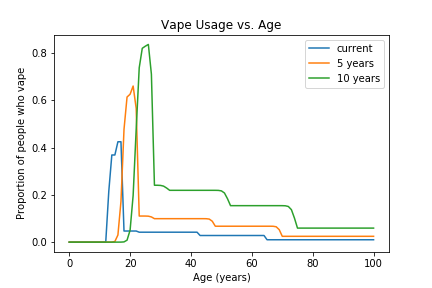
\includegraphics[width=12cm,height=8cm]{figure1.png}\\
\end{center}
\subsection{Justifications}
The change in distribution was calculated using a logistic-like formula. Since the pressure to begin to vape is affected by both people older than you as well as by people your own age, the number of people who begin vaping in a given year can be modeled as 
\[
k*(P(t)+P(t+1))(1-P(t))
\]
where $P(t)$ is the proportion of people who who vape at age $t$, and $k$ is some constant\cite{cdcinfographic}. Note that it is proportional to $1-P(t)$ because the the pressure creates a probability to start, thereby causing more people to start if fewer have already. To create the graph above, $k=0.1$ was used. This thereby models how peer pressure will increase vape usage throughout young age groups, while continuing to increase it among groups that currently vape greatly. This model was calculated using the program in 6.1, the data for which was derived from the data set provided.
\\\\
This prediction ignores the effect of legislation on vaping, and thus may be overestimating the spread of vaping\cite{cdcburdentobacco}. As seen with the 1964 Surgeon General's Report on Smoking and Health\cite{napedu}, cigarette use subsequently over time due to new publicly available information on the harmful effects of vaping on health. It can be assumed that the FDA's recent activity on regulating the use of e-cigarettes such as restricting the sale of flavored versions that appear to target children will have a similar effect\cite{forbestrump}. There may also be a development of a different recreational product that will become widely popular and replace widespread vaping, just as vapes generally replaced the popularity of cigarettes. Although these factors may cause the use of vapes may decrease due to these health concerns, the current social climate and generation of normalized vaping allows the predictions of an increase in use continue to be relevant. 
\newpage

%2nd Question
\section{Episode II: The Attack of the Drugs}
    \subsection{Objective}
    We are asked to create a model that simulates the likelihood of that a given individual will use a given substance. 
    \begin{enumerate}
        \item Predict how many students among a high school class of 300 high school seniors with varying characteristics will use the following substances.
        \begin{itemize}
            \item Nicotine
            \item Marijuana
            \item Alcohol
            \item Unprescribed Opioids
        \end{itemize}
    \end{enumerate}
    \subsection{Local Assumptions}
    \begin{enumerate}
        \item The ratios of given people who are likely to use a given substances are independent of age.
        \item The overdose rate of people are independent of any factors.
        \item{We assume there to be only two genders, male and female.}
    \end{enumerate}
    \subsection{Preliminary Formulas}
    \begin{itemize}
     \item For events $A$ and $B$, $\displaystyle P(A|B)=\dfrac{P(A\cap B)}{P(B)}$
     \\
     \item For events $A$, $B$, and $C$, $P(A\cap B\cap C) \approx \dfrac{P(A \cap B)P(A\cap C)}{P(A)}$
     \end{itemize}
    \subsection{Solution}
        \textbf{Number of Alcohol users}: 89.54065428636922\\
        \textbf{Number of Nicotine users}: 90.94330121091657\\
        \textbf{Number of Marijuana users}: 65.82127566746348\\
        \textbf{Number of Opioids users}: 1.1381565034848171\\
        These numbers were calculated using the calculations described below, using the code in 6.3. The actual mechanics for calculating the probability given certain conditions is using the code in 6.2 as well as the .dat files in 6.4-.6.7. These are calculated by creating a distribution for the 300 students (based on the US averages) and then applying the formulas described. These match almost perfectly with the actual national average of usage among high school seniors. Using the expected values 
    \subsection{Justifications}
    Any general substance can be said to have factors $F_1, F_2, \ldots, F_n$, which are each variables that take on values for any given individual. For example, any substance can be associated with the factors age, race, and income, which may take on a variety of values. Assumption (1) allows us to use general data on consumption of a particular substance to calculate the proportion of all seniors in high school who use the substance, by scaling by a factor of $\dfrac{P(\text{Use drug }|\text{ Senior in HS})}{P(\text{Use drug})}$. Then we can rearrange formulas (1) and (2) in the following manner, where using a particular drug is the event $D$, and the values for the $n$ factors are $V_1, \ldots, V_n$:
    \[
    P(D|V_1\cap V_2 \cap \ldots \cap V_n) = \dfrac{P(D\cap V_1\cap V_2 \cap \ldots \cap V_n)}{P(V_1\cap V_2 \cap \ldots \cap V_n)}
    \]
    Assuming that the factors are approximately independent and repeatedly applying (1)to the numerator yields
    \[
    P(D|V_1\cap V_2 \cap \ldots \cap V_n)=\dfrac{P(D\cap V_1)\ldots P(D\cap V_n)}{P(D)^{n-1}P(V_1)\ldots P(V_n)}
    \]
    Simplifying all pairs of $\dfrac{P(D\cap V_i)}{P(V_i)}=P(D|V_i)$ yields
    \[
    P(D|V_1\cap V_2 \cap \ldots \cap V_n)=\dfrac{1}{P(D)^{n-1}}\Pi_{i=1}^nP(D|V_i)
    \]
    However, all of the values for $P(D|V_i)$ do not account for the age, so applying assumption (1) and using the scaling factor mentioned above yields the final formula, \[
    P(D|V_1\cap V_2 \cap \ldots \cap V_n) = \dfrac{P(D|\text{Senior}}{P(D)^{n-1}}\Pi_{i=1}^nP(D|V_i)
    \]
    \subsection{Data Interpretation}
    The data for the factors of race, gender, and income for each substance were researched and interpreted to be read by the drug\_analysis.py program by formatting them into a .dat file. In each .dat file, the leading value on the first line is the proportion of high school seniors that have used the substance in the past month, and the following lines are groups of 3, where the first line is the category. The line after the category title includes the data subcategories and each value next to the subcategory is the proportion of people in the United States that fit into that category. The next line contains the same subcategories but instead contains proportions of those subcategories that use the substance. These three lines are repeated for different categories. The python program was created to account for varying numbers of categories and subcategories so that the entered data is flexible.
\newpage

%3rd Question
\section{Episode III: Revenge of the Ranks}
\subsection{Objective}
We are asked to develop a robust metric for the impact of substance use taking both financial and non-financial factors and rank the substances mentioned in the previous section.
    
\subsection{Local Assumptions}
\begin{enumerate}
    \item Nicotine was considered to be all tobacco products 
    \item Opioids were considered to be heroine
    \item Data was taken from the a study of the United Kingdom and was applied to the United States
\end{enumerate} 
\subsubsection{Data Table}
{\center
\begin{tabular}{|l|l|l|l|l|}
\hline
\multicolumn{5}{|c|}{\textbf{Data Table 1: Evaluated Statistics}}                                                                 \\ \hline
                                                   & \textbf{Alcohol} & \textbf{Heroin} & \textbf{Nicotine} & \textbf{Marijuana} \\ \hline
\textbf{Loss of Tangibles}                         & 50               & 29               & 10                & 12                 \\ \cline{1-1}
\textbf{Economic Cost}                             & 17               & 5                & 6                 & 4                  \\ \cline{1-1}
\textbf{Drug Specific Mortality}                   & 72               & 55               & 26                & 20                 \\ \cline{1-1}
\textbf{Addiction}                                 & 64               & 100              & 74                & 50                 \\ \cline{1-1}
\textbf{Effect on Others}                          & 74               & 85               & 47                & 50                 \\ \cline{1-1}
\textbf{Physical Harm}                             & 47               & 93               & 41                & 33                 \\ \cline{1-1}
\textbf{Crime}                        & 34               & 20               & 8                 & 7                  \\ \cline{1-1}
\textbf{Average Social Index}                      & 41.66666667      & 36.66666667      & 20.33333333       & 20.33333333        \\ \cline{1-1}
\textbf{Prevalence Multiplier}                     & 0.864            & 0.016            & 0.451             & 0.37               \\ \cline{1-1}
\textbf{Prevalence Multiplier On Societal Impacts} & 36               & 0.5866666667     & 9.170333333       & 7.523333333        \\ \cline{1-1}
\textbf{Average Individual Index}                  & 58.25            & 69.25            & 37.75             & 28.75              \\ \hline
\textbf{Final MEJJJ Index}                               & 94.25            & 69.83666667      & 46.92033333       & 36.27333333        \\ \hline
\end{tabular}
\par}
\subsection{Solution}
    The average of the individual indexes of those subcategories classified as social impacts--Effect on Others, Crime, and Economic Cost--were multiplied by a prevalence multiplier calculated by examining the ubiquity of the four drugs throughout the American population. This approach is modeled by the equation 
    $$\frac{P_m(E_{oO} + C + E_{c})}{3}$$
    The average of the individual indexes of those subcategories classified as individual impacts--Physical Harm, Addiction, Morality, and Crime. These values were not multiplied by a prevalence multiplier as these factors are density-independent and are not affected by the proportion of Americans utilizing the given drugs. This approach to assessing the severity of individual issues is modeled by the equation 
    $$\dfrac{\text{Physical Harm + Addiction + Mortality + Tangibles}}{4}$$ 
    The Average Individual Index was then added to the Average Social Index to yield a Final MEJJJ Index. By placing the four drugs in numerical order with the highest index corresponding with the metric for the greatest impact of the substances and yields an order of Alcohol, Opioids, Nicotine, and Marijuana.

\subsection{Justifications}
    The calculated standings of our Final MEJJJ Index reveals that, on a holistic view of American society, Alcohol is the most prevalent issue regarding the overall population. The combined individual and societal effects of Alcohol outweigh the effects of Opioids, Nicotine, or Marijuana, implying that America’s “deadliest” and most harmful drug is, unsurprisingly, alcohol. The relatively high MEJJJ values for Alcohol and Opioid are valid when considering the realities American culture, which make alcohol and opioids readily available and accessible for potential users at young ages. One strength of the MEJJJ model is the accuracy of the model in relation to American society, where 60\% of underage high school teenagers have had an alcoholic beverage in their lifetime \cite {pubs}. Our model incorporates both holistic and specified analyses for each drug’s areas of influence. Another strength of our model is the comprehensible and simplistic use of the model, which allows for users to simply input the values of another drug to receive the desired drug’s MEJJJ value. One limitation of our model is the inability for the model to factor in for marginal analysis. The model does not account for changes in population and thus does not make accommodations for changes in the prevalence for a given drug. Consequently, our model’s primary use is not to calculate the real impact of substance use using a base year, but is instead useful to assess the impact of substance use for an individual year.

\newpage

\begin{thebibliography}{1}
\bibitem{aspeopioid}
\url{https://aspe.hhs.gov/system/files/pdf/259261/ASPEEconomicOpportunityOpioidCrisis.pdf}
\bibitem{cdcburdentobacco}
\url{https://www.cdc.gov/tobacco/campaign/tips/resources/data/cigarette-smoking-in-united-states.html}
\bibitem{cdcsgeneral}
\url{https://www.cdc.gov/tobacco/data\_statistics/sgr/history/index.htm}
\bibitem{cdcinfographic}
\url{https://www.cdc.gov/vitalsigns/heroin/infographic.html}
\bibitem{cdcnyts}
\url{https://www.cdc.gov/tobacco/data\_statistics/surveys/nyts/data/index.html}
\bibitem{cdcvital}
\url{https://www.cdc.gov/mmwr/preview/mmwrhtml/mm6452a3.htm}
\bibitem{cnbcteencig}
\url{https://www.cnbc.com/2018/10/22/teen-cigarette-smoking-ticks-up-as-vaping-surges.html}
\bibitem{gallupalcoholdrink}
\url{https://news.gallup.com/poll/1582/Alcohol-Drinking.aspx}
\bibitem{gallupalcoholincome}
\url{https://news.gallup.com/poll/184358/drinking-highest-among-educated-upper-income-americans.aspx}
\bibitem{galluptobacco}
\url{https://news.gallup.com/poll/237839/americans-say-marijuana-vaping-less-harmful-tobacco.aspx?g\_source=link\_newsv9&g\_campaign=item\_237818&g\_medium=copy}
\bibitem{galluptrymari}
\url{https://news.gallup.com/poll/214250/say-tried-marijuana.aspx}
\bibitem{gallupyoungpeople}
\url{https://news.gallup.com/poll/237818/young-people-adopt-vaping-smoking-rate-plummets.aspx}
\bibitem{infoplease}
\url{https://www.infoplease.com/science-health/health/smoking-prevalence-among-us-adults-1955a2013}
\bibitem{jamanetwork}
\url{https://jamanetwork.com/journals/jama/fullarticle/2428954?resultClick=3}
\bibitem{monitoringfuture}
\url{http://monitoringthefuture.org/pubs/monographs/mtf-overview2015.pdf}
\bibitem{statisaperadult}
\url{https://www.statista.com/statistics/261576/cigarette-consumption-per-adult-in-the-us/}
\bibitem{statisasmoking}
\url{https://www.statista.com/topics/1600/smoking/}
\bibitem{narconon}
\url{https://www.narconon.org/blog/drug-use/does-race-gender-or-ethnicity-determine-drug-use/}
\bibitem{napedu}
\url{https://www.nap.edu/read/11795/chapter/4\#42}
\bibitem{ncbi}
\url{https://www.ncbi.nlm.nih.gov/pmc/articles/PMC4644488/}
\bibitem{ncbigenderopi}
\url{https://www.ncbi.nlm.nih.gov/pmc/articles/PMC3164783/}
\bibitem{ncbiagetable}
\url{https://www.ncbi.nlm.nih.gov/books/NBK294302/table/ch13.t2/?report=objectonly}
\bibitem{ncbihistoricaltrend}
\url{https://www.ncbi.nlm.nih.gov/books/NBK294302/table/ch13.t2/?report=objectonly}
\bibitem{ncbiincomepat}
\url{https://www.ncbi.nlm.nih.gov/pmc/articles/PMC3185179/}
\bibitem{ncbialcoconsumption}
\url{https://www.ncbi.nlm.nih.gov/pmc/articles/PMC4872616/}
\bibitem{ncbimarijuana}
\url{https://www.ncbi.nlm.nih.gov/pmc/articles/PMC3410945/}
\bibitem{nprhabits}
\url{https://www.npr.org/sections/health-shots/2015/03/17/393554628/income-affects-how-genes-play-a-role-in-drinking-problems}
\bibitem{samhsa}
\url{https://www.samhsa.gov/data/nsduh/reports-detailed-tables-2017-NSDUH}
\bibitem{vizhub}
\url{https://vizhub.healthdata.org/tobacco/}
\bibitem{ukdrugharms}
\url{http://www.ias.org.uk/uploads/pdf/news\%20stories/dnutt-lancet-011110.pdf}
\bibitem{researchgate}
\url{https://www.researchgate.net/publication/6424313\_Development\_\of\_\a\_rational\_scale\_to\_assess\_the\_harm\_of\_drugs\_of\_potentia\l_misuse}

\bibitem{forbestrump}
\url{https://www.forbes.com/sites/tomangell/2017/09/25/trump-administration-makes-it-harder-to-track-marijuana-arrests-but-i-did-it-anyway/#5295f9e468bc}

\bibitem{alcrehab}
\url{https://www.alcoholrehabguide.org/alcohol/crimes/}

\bibitem{drugwarfacts}
\url{https://www.drugwarfacts.org/chapter/crime\_arrests}

\bibitem{niaalcohol}
\url{https://www.niaaa.nih.gov/alcohol-health/overview-alcohol-consumption/alcohol-facts-and-statistics}

\bibitem{jamanet}
\url{https://jamanetwork.com/journals/jamapsychiatry/fullarticle/2612444} 

\bibitem{omicsonline}
\url{https://www.omicsonline.org/lifetime-and-current-prevalence-of-tobacco-smoking-2155-6105.1000145.php?aid=14160}
\bibitem{pubs}
\url{https://pubs.niaaa.nih.gov/publications/UnderageDrinking/UnderageFact.htm}
\bibitem{given}
\url{https://mym3challenge.siam.org/the-problem}
\end{thebibliography}
\newpage

\section{Appendix}
\subsection{spread.py: Calculating the spread of Vape Usage}
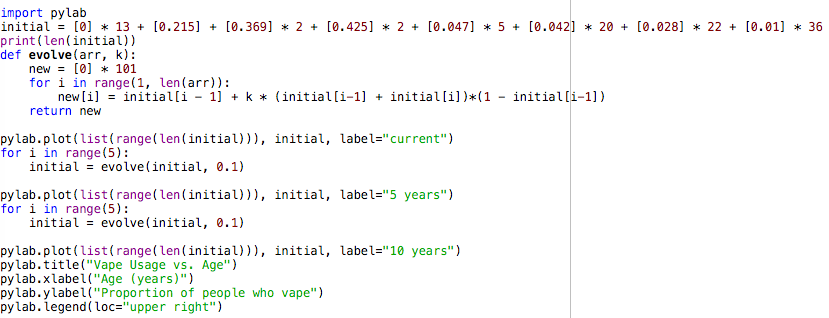
\includegraphics[width=\textwidth]{spread}
\subsection{drug\_analysis.py: Calculating the probability of using a substance}
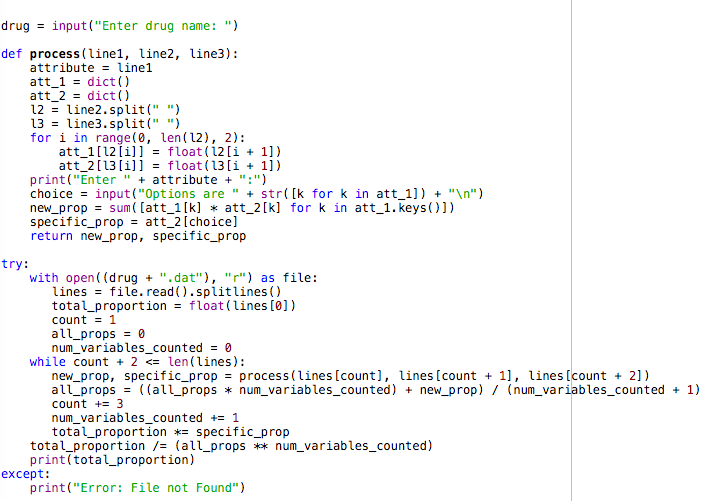
\includegraphics[width=\textwidth]{druganalysis.png}
\subsection{all\_students.py: Calculating expected numbers in a class of 300}
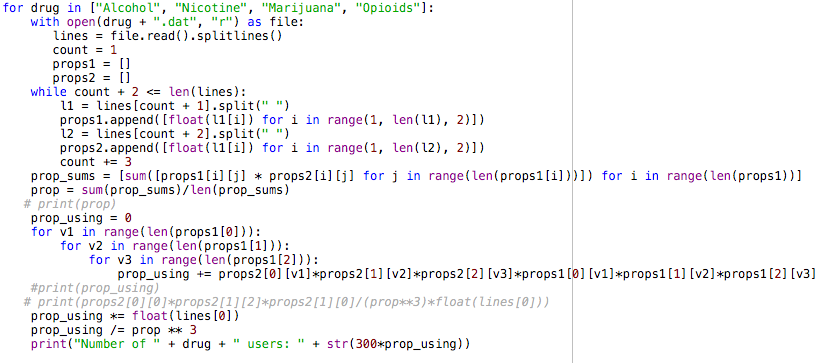
\includegraphics[width=\textwidth]{class.png}
\subsection{Alcohol.dat}
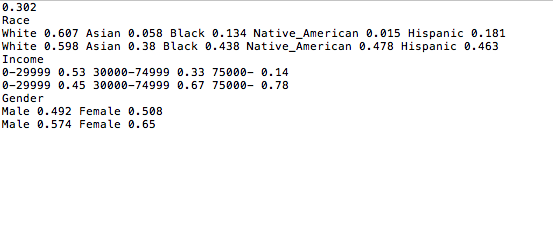
\includegraphics{alc.png}
\subsection{Marijuana.dat}
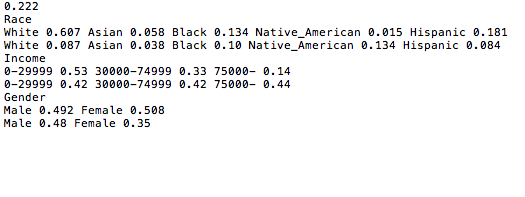
\includegraphics{mar.png}
\subsection{Opioids.dat}
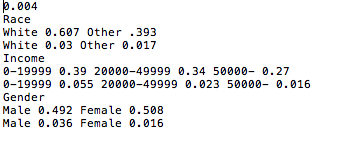
\includegraphics{opi.png}
\subsection{Nicotine.dat}
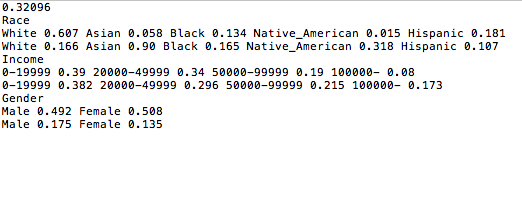
\includegraphics{nico.png}
\end{document}
